\documentclass{article}
\title{Matrix Equation Solvers}
\author{Alex Harvey - mm13ah - ID: 200786528}
\date{}

\usepackage{amsmath}
\numberwithin{equation}{section}
\usepackage{amssymb}
\usepackage{amsthm}
\usepackage{blindtext}
\usepackage[parfill]{parskip}
\usepackage{graphicx}
\usepackage{textcomp}
\usepackage[utf8]{inputenc}
\usepackage{float}
\usepackage{diagbox}
\usepackage{tikz}
\usepackage{pgfgantt}
\usepackage{nicefrac}

\begin{document}

\maketitle
\section{Introduction}

The traditional approach to solving PDEs numerically involves stacking all unknowns of the problem into a single vector which ignores underlying structures. This prevents methods from being used which can take advantage of the problem structure to solve the problem more efficiently. An alternative approach is to formulate the problem as a matrix equation, which can be solved using a range of different methods. This project involves exploring how this alternative formulation can be solved using matrix solvers, and how these solvers compare against each other. As an example, let $u: \Omega \to \mathbb{R}$. Then let the equation:
	\begin{equation} 
	-u_{xx} - u_{yy} = f
	\end{equation}
be defined on $\Omega = (0,1) \times(0,1)$, with boundary conditions $u(x,y)=0$, as shown below:

\begin{figure}[H]
\begin{tikzpicture}
\draw (0,0) rectangle (6,6);
\node at (3,3) {$-u_{xx}-u_{yy}=f$};
\node at (-0.25,3) {$0$};
\node at (6.25,3) {$0$};
\node at (3,-0.25) {$0$};
\node at (3,6.25) {$0$};

\node at (-0.25,-0.25) {$(0,0)$};
\node at (-0.25,6.25) {$(0,1)$};
\node at (6.25,-0.25) {$(1,0)$};
\node at (6.25,6.25) {$(1,1)$};

\draw[->] (7,0) -- (8,0);
\draw[->] (7,0) -- (7,1);
\node at (7.5,-0.25) {$x$};
\node at (6.75,0.5) {$y$};
\end{tikzpicture}
\centering
\caption{Domain for $-u_{xx}-u_{yy}=f$}
\end{figure}

The domain of this PDE can be discretised into a mesh with uniform spacing $h$ using the centred finite difference approximations:
	\begin{equation} 
	u_{xx} \approx \frac{u_{i-1j} - 2u_{ij} + u_{i+1j}}{h^2}
	\end{equation}
	\begin{equation}
	u_{yy} \approx \frac{u_{ij-1} - 2u_{ij} + u_{ij+1}}{h^2}
	\end{equation}
where $u_{ij} = u(x_i, y_j)$. The mesh is shown below:

\begin{figure}[H]
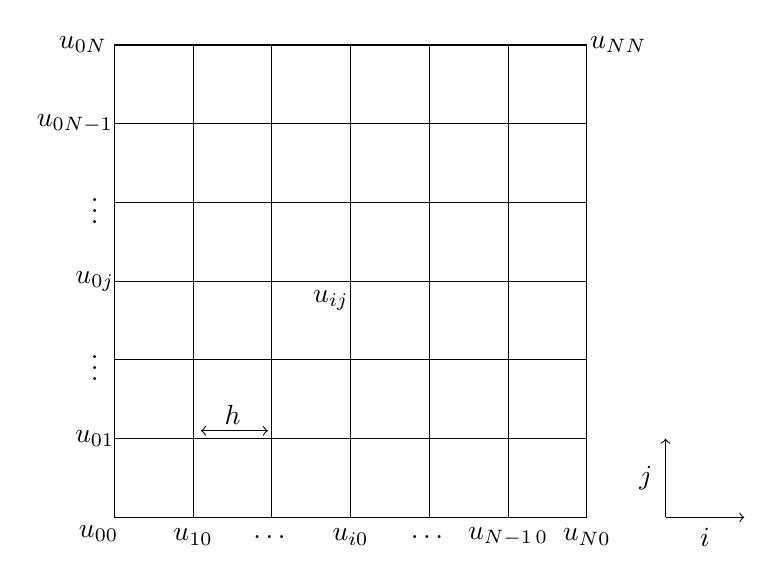
\begin{tikzpicture}
\draw (0,0) grid (6,6);
\node at (-0.2,-0.2) {$u_{00}$};
\node at (1,-0.25) {$u_{10}$};
\node at (2,-0.25) {$\dots$};
\node at (3,-0.25) {$u_{i0}$};
\node at (4,-0.25) {$\dots$};
\node at (5,-0.25) {$u_{N-1\,0}$};
\node at (6,-0.25) {$u_{N0}$};

\node at (-0.25,1) {$u_{01}$};
\node at (-0.25,2) {$\vdots$};
\node at (-0.25,3) {$u_{0j}$};
\node at (-0.25,4) {$\vdots$};
\node at (-0.5,5) {$u_{0N-1}$};
\node at (-0.4,6) {$u_{0N}$};

\node at (2.75,2.75) {$u_{ij}$};
\node at (6.4,6) {$u_{NN}$};

\draw[->] (7,0) -- (8,0);
\draw[->] (7,0) -- (7,1);
\node at (7.5,-0.25) {$i$};
\node at (6.75,0.5) {$j$};

\draw[<->] (1.1,1.1) -- (1.95,1.1);
\node at (1.5,1.3) {$h$};

\end{tikzpicture}
\centering
\caption{Discretised domain for $-u_{xx}-u_{yy}=f$}
\end{figure}

The discretised form of this PDE can then be solved by computing the equation:
	\begin{equation}
	f_{ij} = -\frac{1}{h^2} \big( u_{i-1j} - 2u_{ij} + u_{i+1j} \big) - \frac{1}{h^2} \big( u_{ij-1} - 2u_{ij} + u_{ij+1} \big)
	\end{equation}
at each internal grid point, meaning the system has $n^2$ unknowns with $n=N-2$. The traditional approach to solving this discretised form would be to write (1.4) as:
	\begin{equation}
	f_{ij} = -\frac{1}{h^2} \big( u_{i-1j} + u_{ij-1} - 4u_{ij} + u_{i+1j} + u_{ij+1}  \big)
	\end{equation}
and then stack all unknowns $u_{ij}$ into a single vector $U$, resulting in the linear system $AU=F$. As stated, this ignores the underlying structure of the problem.

By keeping (1.4) in its original form we can instead write the system as a matrix equation:
	\begin{equation} 
	TU + UT = F
	\end{equation}
with $T=-\frac{1}{h^2} \, \text{tridiag}(1,-2,1)$ and $U_{ij} = u(x_i, y_j)$ where $(x_i, y_j)$ are interior grid nodes for $i,j=1,\dots,n$. This equation is in the form of a Sylvester equation $AX + XB = C$, with $A=B=T$, $X=U$ and $C=F$, and there many different methods that can be used to solve equations of this type. This project will explore different methods for solving equations in this form. 

\newpage

\section{Scope and Schedule}
\subsection{Aim}
The aim of this project is to first study, implement and compare a range of matrix equation solvers. Following this, a specific problem will be derived with the help of my supervisor so that these solvers may be used and compared for a suitable application.

\subsection{Objectives}
The objectives of this project are as follows:
\begin{itemize}
\item To carry out an extensive, in-depth literature review on methods (both iterative and direct) for solving matrix equations from a wide range of sources. To decide which of these methods are appropriate to implement and to gain a solid understanding of how they work. 
\item To use and expand upon my programming experience to implement the chosen methods for solving matrix equations to solve the specified problem. 
\item To evaluate the implementation by comparing and contrasting the methods implemented to try to decide which is the best method for solving the given problem.
\item To derive a suitable application equation so that the methods studied in this project can be applied to a specific problem. 
\item To clearly present the work carried out during the project by using and building upon my report writing skills.
\end{itemize}

\subsection{Deliverables}
The deliverables of this project include:
\begin{itemize}
\item The final report that will include the details of the matrix solvers that have been studied, how the solvers were implemented, an evaluation and comparison of the implemented solvers, an analysis of how these solvers were used to solve the chosen application problem, and finally an evaluation of the success of the project.  
\item Code that successfully implements the chosen matrix solvers so that they solve the given problem.
\end{itemize}

\subsection{Methodology}
The methodology of this project will first involve studying academic publishings to gain an understanding of various methods for solving matrix equations. Python will be used as the programming language of choice for the implementation because of my familiarity with it, the extensive amount of documentation available for it and the excellent libraries it has available (e.g. NumPy and SciPy). GitHub will be used for version control and the final report will be written using \LaTeX. 

\subsection{Tasks, milestones and timeline}
The steps of this project will be divided into iterations, with the problem in each iteration becoming successively more complex and difficult to solve. This is because understanding is a key part of this project, and so each iteration will build on the understanding of the last. Each iteration will consist of studying and applying matrix methods to the problem, implementing them in Python to solve the problem, evaluating the results and write up. Also rough deadlines will be given for when each iteration should be completed by, to ensure the project is on track at any given stage.

The iterations are as follows:
\begin{itemize}
\item Introductory problem: $-u_{xx} - u_{yy} = 2 \pi^2 \sin{(\pi x)} \sin{(\pi y)}$ - deadline June 1st
\item Problem introducing uncertainty: $-\varepsilon u_{xx} - \varepsilon u_{yy} = 2 \pi^2 \sin{(\pi x)} \sin{(\pi y)}$ - deadline June 22nd
\item A Poisson equation on a surface defined by a height map (not yet derived) - deadline July 13th
\item Application reaction-diffusion equation (not yet derived) - deadline August 3rd
\end{itemize}

If the project deadlines are met the remaining time will be dedicated to project evaluation, write up and any possible project extensions.

\newpage

\section{Matrix Solvers}
As an example problem, let the exact solution, $u$, of (1.1) be defined as:
\begin{equation} 
u = \sin{(\pi x)} \sin{(\pi y)}
\end{equation}
which gives:
\begin{equation} 
u_{xx} = u_{yy} = - \pi^2 \sin{(\pi x)} \sin{(\pi y)}
\end{equation}
\begin{equation}
\implies F = 2 \pi^2 \sin{(\pi x)} \sin {(\pi y)}
\end{equation}
The PDE to be solved is now:
\begin{equation}
-u_{xx} - u_{yy}  = 2 \pi^2 \sin{(\pi x)} \sin {(\pi y)}
\end{equation}
at each grid point, or equivalently:
	\begin{equation}
	TU + UT = F
	\end{equation}
as a matrix equation. Here $T=-\frac{1}{h^2} \, \text{tridiag}(1,-2,1)$, $U_{ij} = u(x_i, y_j)$ and $F_{ij} = 2 \pi^2 \sin{(\pi x_i)} \sin{(\pi y_j)}$, where $(x_i, y_j)$ are interior grid nodes for $i,j=1,\dots,n$. As stated previously this equation is in the form of a Sylvester equation and can be solved using a range of different methods. A graph of the exact solution, with $n=1000$, is given below:

\begin{figure}[H]
\includegraphics[scale=.7]{img/U_sol.png}
\centering
\end{figure} 

Throughout the following section, the following measurements are given to evaluate the performance of each of the methods implemented:
\begin{itemize}
\item $n$: The total number of unknowns for the system.
\item Time(s): The time taken in seconds for the method to compute the solution to the problem.
\item L$_{\text{max}}$: Measures the maximum difference between the actual solution and computed solution for each $u$, defined as:
 \[ || u - u_h ||_{L^\infty} = \text{max}_{ij} | u(x_i, y_i) - u_{ij} | \]
\item L$_{\text{squared}}$: A measure of error that takes into account the difference between all actual and computed solutions, as well as the step size. Defined as:
\[ || u - u_h ||_{L^2} = \sqrt{h^2 \sum | u(x_i,y_j) - u_{ij} |^2} \]
\item Experimental order of convergence: Measures the rate of convergence of a method, which should approach 2 as the step size is increased. Defined as:
\[ \text{eoc}(i) = \frac{\log{(\nicefrac{E_i}{E_{i-1}})}}{\log{(\nicefrac{h_i}{h_{i-1}})}} \]
where $E_i$ is the error and $h_i$ is the mesh size at level $i$. 
\end{itemize}

\subsection{Direct Methods}

\subsubsection{Kronecker Product}
A naive approach to solving this system is to use the Kronecker product to rewrite (3.5) as a standard vector linear system. The Sylvester equation $AX + XB = C$ can be written as the standard vector linear system:
\begin{equation}
\mathcal{A}x = c
\end{equation}
with $\mathcal{A} = I \otimes A + B^* \otimes I$, where $I$ is the identity matrix, $B^*$ denotes the conjugate transpose of $B$, $x = \text{vec}(X)$ and $c = \text{vec}(C)$.\footnote{The vec operator reshapes a matrix into a vector by stacking the columns one after another.}

For the system in (3.6), we have $A=B=T$, $X=U$, $C=F$ and $T=T^*$, so the standard linear system is:
\begin{equation}
\mathcal{T}u = \mathcal{F}
\end{equation}
where $\mathcal{F}$ is a vector of dimension $n^2$, $\mathcal{T} = I \otimes T + T \otimes I$ and $u = \text{vec}(U)$. 

This is the exact linear system that would be obtained from equation (1.5), i.e. stacking all unknowns $u_{ij}$ into a single vector in the first place. Since the matrix $\mathcal{T}$ is sparse, this equation can be solved using a standard direct sparse solver. This approach provides a good base case for comparison. Results solving this linear system using the direct sparse solver \texttt{sparse.linalg.spsolve} from the SciPy library are given below:

\begin{figure}[H]
\includegraphics[scale=.7]{img/U_sparse.png}
\centering
\end{figure}

\begin{table}[H]
\centering
\begin{tabular}{|c|c|c|c|c|}
\hline
$n$ & Time(s) & $|| u - u_h ||_{L^{\infty}}$ &$|| u - u_h ||_{L^{2}}$ & eoc \\
\hline
10 & 0.0026031 & 0.0066868 & 0.0034125 & - \\
100 & 0.061922 & 8.0611e$^{-5}$ & 4.0315e$^{-5}$ & 1.9927 \\
1000 & 36.681 & 8.2082e$^{-7}$ & 4.1041e$^{-7}$ & 1.9999  \\
2000 & 428.06 & 2.0540e$^{-7}$ & 1.0270e$^{-7}$ & 2.0001 \\
\hline
\end{tabular}
\end{table}

\subsubsection{Bartels-Stewart Algorithm}
The Bartels-Stewart algorithm \cite{Bartels} can be used to solve the Sylvester equation $AX + XB = F$. In the general case the algorithm is as follows:
\begin{enumerate}
\item Compute the Schur forms $A^* = PRP^*$ and $B=QSQ^*$
\item Solve $R^*V + VS = P^*FQ$ for $V$
\item Compute $X=PVQ^*$
\end{enumerate}
where $A^*$ denotes the conjugate transpose of $A$.

In this case $A=B=T$, $T=T^*$ and $X=U$, so the algorithm is as follows:
\begin{enumerate}
\item Compute the Schur form $T=PRP^*$
\item Solve $R^*V + VR = P^*FP$ for $V$
\item Compute $U=PVP^*$
\end{enumerate}

Results using this algorithm are given below:

\begin{figure}[H]
\includegraphics[scale=.7]{img/U_bartels.png}
\centering
\end{figure}

\begin{table}[H]
\centering
\begin{tabular}{|c|c|c|c|c|c|}
\hline
$n$ & Time(s) & $|| u - u_h ||_{L^{\infty}}$ &$|| u - u_h ||_{L^{2}}$ & eoc \\
\hline
10 & 0.0076599 & 0.0066868 & 0.0034125 & - \\
100 & 2.0357 & 8.0611e$^{-5}$ & 4.0315e$^{-5}$ & 1.9927 \\
1000 & 1449.6 & 8.2083e$^{-7}$ & 4.1041e$^{-7}$ & 1.9999 \\
2000 & 8675.8 & 2.0561e$^{-7}$ & 1.0276e$^{-7}$ & 1.9986 \\
\hline
\end{tabular}
\end{table}

The SciPy library has a built in solver for solving Sylvester equations, \texttt{scipy.linalg solve\_sylvester}, which uses the Bartels-Stewart algorithm. Results using this solver are given below:

\begin{figure}[H]
\includegraphics[scale=.7]{img/U_scipy.png}
\centering
\end{figure}

\begin{table}[H]
\centering
\begin{tabular}{|c|c|c|c|c|}
\hline
$n$ & Time(s) & $|| u - u_h ||_{L^{\infty}}$ &$|| u - u_h ||_{L^{2}}$ & eoc \\
\hline
10 & 0.00051880 & 0.0066868 & 0.0034125 & -  \\
100 & 0.027365 & 8.0611e$^{-5}$ & 4.0315e$^{-5}$ & 1.9927  \\
1000 & 20.248 & 8.2083e$^{-7}$ & 4.1041e$^{-7}$ & 1.9999 \\
2000 & 244.27 & 2.0558e$^{-7}$ & 1.0277e$^{-7}$ & 1.9988  \\
4000 & 2886.7 & 5.0158e$^{-8}$ & 2.4922e$^{-8}$ & 2.0359 \\
%5000 & 6133.9 & 4.3474e$^{-8}$ & 2.1236e$^{-8}$ & 1.6962  \\
\hline
\end{tabular}
\end{table}

As can be seen from the results above, using the built-in SciPy solver results in a significant speed-up in time as $n$ is increased. This is likely because it makes use of of LAPACK, which is an optimised software library for solving linear algebra problems.


\subsubsection{Similarity Transformations}
A similarity transformation \cite{Simoncini} can be used to solve the Sylvester equation $AX + XB = F$, where $A$ is a $n \times n$ matrix and $B$ is a $m \times m$ matrix. 

Assuming matrices $A$ and $B$ can be diagonalised, let $P^{-1}AP = \text{diag}(\lambda_1, \dots, \lambda_n)$ and $Q^{-1}BQ = \text{diag}(\mu_1, \dots, \mu_m)$, where $\lambda_1, \dots, \lambda_n$ are the eigenvalues of $A$ and $\mu_1, \dots, \mu_m$ are the eigenvalues values of $B$. Let $\tilde{F} = P^{-1}FQ$. The solution is then:
\[ X = P \tilde{X} Q^{-1}, \text{ with } \tilde{x}_{ij} = \frac{\tilde{f}_{ij}}{\lambda_i + \mu_j} \]

In this case, $A=B=T$ and $X=U$, so $P=Q$ and $P^{-1}TP = \text{diag}(\lambda_1, \dots, \lambda_n)$, where $\lambda_1, \dots, \lambda_n$ are the eigenvalues of $T$. Also $\tilde{F}=P^{-1}FP$. The solution is therefore:
\[ U = P \tilde{U} P^{-1}, \text{ with } \tilde{u}_{ij} = \frac{\tilde{f}_{ij}}{\lambda_i + \lambda_j} \]

\subsubsection*{Using numpy.linalg.eig}
The eigenvalues and eigenvectors can be computed using NumPy's \texttt{linalg.eig} function. The results using this are given below:

\begin{figure}[H]
\includegraphics[scale=.7]{img/U_trans.png}
\centering
\end{figure}

\begin{table}[H]
\centering
\begin{tabular}{|c|c|c|c|c|}
\hline
$n$ & Time(s) & $|| u - u_h ||_{L^{\infty}}$ &$|| u - u_h ||_{L^{2}}$ & eoc \\
\hline
10 & 0.023603 & 0.0066868 & 0.0034125 & - \\
100 & 0.049893 & 8.0611e$^{-5}$ & 4.0315e$^{-5}$ & 1.9927  \\ 
1000 & 4.8863 & 8.2083e$^{-7}$ & 4.1041e$^{-7}$ & 1.9999  \\
2000 & 26.098 & 2.0560e$^{-7}$ & 1.0277e$^{-7}$ & 1.9987 \\
4000 & 185.13 & 5.0151e$^{-8}$ & 2.4922e$^{-8}$ & 2.0362 \\
8000 & 1274.5 & 1.2959e$^{-8}$ & 5.1767$^{-9}$ & 1.9527 \\
%5000 & 265.25 & 4.3041e$^{-8}$ & 2.1164e$^{-8}$ & 1.7072 \\
%10000 & 2019.2 & 1.5349e$^{-9}$ & 6.8831e$^{-9}$ & 4.8102 \\
\hline
\end{tabular}
\end{table}

Here the experimental order converges moves away from 2 as $n$ is increased. This is likely due to the fact that as there is no general formula for calculating eigenvalues and eigenvectors, the eigenvalues and eigenvectors are approximated by NumPy's \texttt{linalg.eig}.

This method can be split into component parts and each part can be timed, to see which part is the most costly. The steps of the method are:
\begin{enumerate}
\item Calculate eigenvalues and eigenvectors of $T$
\item Diagonalise $T$ (i.e. calculate $P$ and $P^{-1}$)
\item Calculate $\tilde{F}=P^{-1}FP$
\item Calculate $\tilde{U}$, where $\tilde{u}_{ij} = \frac{\tilde{f}_{ij}}{\lambda_i + \lambda_j}$
\item Calculate solution $U=P \tilde{U}P^{-1}$
\end{enumerate}

The results of doing so are given below:

\begin{table}[H]
\centering
\begin{tabular}{|c|c|c|c|c|c|c|}
\hline
$n$ & 1 & 2 & 3 & 4 & 5 & Total \\
\hline
10 & 0.0057750 & 0.0045397 & 0.0010521 & 0.011951 & 0.00028515 & 0.023603 \\
100 & 0.024929 & 0.0011380 & 0.0017610 & 0.020651 & 0.0014130 & 0.049893 \\
1000 & 2.5253 & 0.070281 & 0.21545 & 1.8795 & 0.19585 & 4.8863 \\
2000 & 15.457 & 0.0056458 & 1.5614 & 7.5858 & 1.4880 & 26.098 \\
4000 & 121.16 & 0.060127 & 12.136 & 39.220 & 12.557 & 185.13 \\
8000 & 922.39 & 0.04993 & 102.79 & 131.24 & 118.03 & 1274.5  \\
%5000 & 172.85 & 0.022033 & 23.074 & 48.185 & 21.110 & 265.25 \\
%10000 & 1422.9 & 0.07697 & 189.07 & 191.39 & 215.76 & 2019.2 \\
\hline
\end{tabular}
\end{table}

\subsubsection*{Calculating eigenvalues and eigenvectors explicitly}

As can be seen from the results above, the most costly part of this method is calculating the eigenvalues and eigenvectors. As $T$ is a matrix in Toeplitz form, the eigenvalues and eigenvectors can be calculated directly as:
\[ \lambda_i = \frac{2}{h^2} \Big( \cos \Big( \frac{i \pi}{n+1} \Big) - 1 \Big) \]
and 
\[ t_{ij} = \sqrt{\frac{2}{n+1}} \sin \Big( \frac{ij \pi}{n+1}  \Big) \]

Results using this method for calculating the eigenvalues are eigenvectors are given below:

\begin{figure}[H]
\includegraphics[scale=.7]{img/U_trans2.png}
\centering
\end{figure}

\begin{table}[H]
\centering
\begin{tabular}{|c|c|c|c|c|}
\hline
$n$ & Time(s) & $|| u - u_h ||_{L^{\infty}}$ &$|| u - u_h ||_{L^{2}}$ & eoc \\
\hline
10 & 0.0041900 & 0.0066868 & 0.0034125 & - \\
100 & 0.076722 & 8.0610e$^{-5}$ & 4.0315e$^{-5}$ & 1.9927 \\
1000 & 7.0524 & 8.2082e$^{-7}$ & 4.1041e$^{-7}$ & 1.9999 \\
2000 & 29.164 & 2.0541e$^{-7}$ & 1.0270e$^{-7}$ & 2.0000 \\
4000 & 103.42 & 5.1313e${-8}$ & 2.5655e$^{-8}$ & 2.0018 \\
8000 & 593.77 & 1.2814e$^{-8}$ & 6.4065e$^{-9}$ & 2.0020 \\
%5000 & 224.29 & 3.3196e$^{-8}$ & 1.6598e$^{-8}$ & 1.9897 \\
%10000 & 1190.3 & 8.2857e$^{-9}$ & 4.1418e$^{-9}$ & 2.0026 \\
\hline
\end{tabular}
\end{table}

\begin{table}[H]
\centering
\begin{tabular}{|c|c|c|c|c|c|c|}
\hline
$n$ & 1 & 2 & 3 & 4 & 5 & Total \\
\hline
10 & 0.00089598 & 0.00071597 & 0.0014319 & 0.00087380 & 0.00027227 & 0.0041900 \\
100 & 0.047597 & 0.00061584 & 0.0015020 & 0.0.025820 & 0.0011868 & 0.076722 \\
1000 & 4.1079 & 0.0032451 & 0.23045 & 2.4986 & 0.21222 & 7.0524 \\
2000 & 16.395 & 0.063026 & 1.4521 & 9.8474 & 1.4060 & 29.164 \\
4000 & 52.499 & 0.034972 & 10.389 & 28.196 & 12.305 & 103.42 \\
8000 & 238.04 & 0.12201 & 113.94 & 132.86 & 108.81 & 593.77 \\
%5000 & 114.13 & 0.020910 & 23.862 & 62.216 & 24.068 & 224.29 \\
%10000 & 416.39 & 0.088258 & 227.01 & 302.53 & 244.27 & 1190.3 \\
\hline
\end{tabular}
\end{table}

As can be seen from the results above, calculating the eigenvalues and eigenvectors explicitly vastly outperforms calculating them using the NumPy library when $n$ is large.

\subsection{Iterative Methods}

\subsubsection{Kronecker Product}
Similarly to Section 3.1.1, the Kronecker product can be used to write the matrix equation as a standard vector linear system. A a standard iterative solver can then be used to solve the system, which can provide a base case for comparison. Results using \texttt{scipy.sparse.linalg.cg}, which is a sparse solver that uses the conjugate gradient iterative method, are given below, using a convergence tolerance of 1be$^{-9}$.

\begin{table}[H]
\centering
\begin{tabular}{|c|c|c|c|c|}
\hline
$n$ & Time(s) & $|| u - u_h ||_{L^{\infty}}$ &$|| u - u_h ||_{L^{2}}$ & eoc \\
\hline
10 & 0.0023940 & 0.0066868 & 0.0034124 & - \\
100 & 0.0048580 & 8.0611e$^{-5}$ & 4.0315e$^{-5}$ & \\
1000 & 0.61869 & 8.2082e$^{-7}$ & 4.1041e$^{-7}$ & \\
2000 & 2.1425 & 2.0541e$^{-7}$ & 1.0271e$^{-7}$ & \\
4000 & 23.065 & 5.1378e$^{-8}$ & 2.5689e$^{-8}$ & \\
8000 & 160.09 & 1.2848e$^{-8}$ & 6.4239e$^{-9}$ & \\
\hline
\end{tabular}
\end{table}

\subsubsection{Gradient based method}
In \cite{Zhou} a gradient based method for solving Sylvester equations is proposed. The equation $TU + UT = F$ can be written as two recursive sequences:
	\begin{equation}
	U_k^{(1)} = U_{k-1}^{(1)} + \kappa T(F-TU_{k-1}^{(1)} - U_{k-1}^{(1)}T)
	\end{equation}
	\begin{equation}
	U_k^{(2)} = U_{k-1}^{(2)} + \kappa (F-TU_{k-1}^{(2)} - U_{k-1}^{(2)}T)T
	\end{equation}
where $\kappa$ represents the relative step size. The approximate solution $U_k$ is taken as the average of these two sequences:
	\begin{equation}
	U_k = \frac{U_k^{(1)} + U_k^{(2)}}{2}
	\end{equation}
This solution only converges if:
	\begin{equation}
	0 < \kappa < \frac{1}{\lambda_{\text{max}}(T^2)} 
	\end{equation}
where $\lambda_{\text{max}}(T^2)$ denotes the maximum eigenvalue of $T^2$. Using the method given previously for calculating eigenvalues we can compute:
\begin{equation}
\lambda_{\text{max}}(T^2) = \frac{4}{h^4} \text{max} \Big( \big( \cos{\Big(\frac{i \pi}{n+1} \Big) } -1 \big)^2 \Big)
\end{equation}
$\lambda_{\text{max}}(T^2)$ therefore scales with $\frac{1}{h^4}$ meaning its reciprocal scales with $h^4$, implying $\kappa$ will need to be significantly small as $n$ is increased for the solution to converge. Even for small values of $n$, this is impractical and therefore this method is not appropriate for solving this equation.






%\begin{itemize}
%\item Naive approach \cite{Simoncini}: (1.6) can be written in the form of a standard linear system:
%	\begin{equation}
%	\mathcal{T}u = \mathcal{F}
%	\end{equation}
%where $\mathcal{F}$ is a vector of dimension $n^2$, $\mathcal{T} = I \otimes T + T \otimes I$ and $u = \text{vec}(U)$. Here $\otimes$ denotes the Kronecker product and vec is an operator that reshapes a matrix into a vector by stacking the columns one after another. 
%This is the exact linear system that would be obtained from equation (1.5), i.e. stacking all unknowns $u_{ij}$ into a single vector in the first place. Since the matrix $\mathcal{T}$ is sparse, this equation can be solved using a standard sparse iterative or direct solver (e.g. \texttt{sparse.linalg.spsolve} from the SciPy library). This approach provides a good base case for comparison.
%\item Bartels-Stewart algorithm \cite{Bartels} \cite{Simoncini}: A common algorithm for solving Sylvester equations is the Bartels-Stewart algorithm. This algorithm transforms (1.6) into a simpler but equivalent problem by computing the Schur decomposition of $T$ so that the resulting matrices are lower/upper triangular. The resulting unknown matrix can then be solved sequentially and the solution $U$ can be computed. The algorithm is as follows:
%	\begin{enumerate}
%	\item Compute the Schur form $T=PRP^*$
%	\item Solve $R^*V + VR = P^*FP$ for $V$
%	\item Compute $U=PVP^*$
%	\end{enumerate}
%where $P^*$ denotes the conjugate transpose of $P$. The SciPy library has a built-in  solver for solving Sylvester equations, \texttt{linalg.solve\_sylvester}, which uses this algorithm.
%\item Similarity transformations \cite{Simoncini}: This approach assumes that the matrix $T$ can be diagonalised in the form $P^{-1}TP = \text{diag}(\lambda_1, \dots, \lambda_n)$, where $\lambda_1, \dots, \lambda_n$ denote the eigenvalues of $T$. Here the columns of $P$ are the eigenvectors of $T$. By computing the matrix $\tilde{F} = P^{-1}FP$, the solution can be computed as:
%	\begin{equation}
%	U = P \tilde{U} P^{-1}, \; \text{ with } \tilde{u}_{ij} = \frac{\tilde{f}_{ij}}{\lambda_i + \lambda_j}
%	\end{equation}
%The eigenvalues and eigenvectors of $T$ can be computed using, for example, \texttt{linalg.eig} from the NumPy library, or can alternatively be computed explicitly as:
%	\begin{equation}\lambda_i = \frac{2}{h^2} \Big( \cos \Big( \frac{i \pi}{n+1} \Big) - 1 \Big)
%	\end{equation}
%	\begin{equation}
%	t_{ij} = \sqrt{\frac{2}{n+1}} \sin \Big( \frac{ij \pi}{n+1}  \Big) 
%	\end{equation}
%which leads to a significant speed up in time for large $n$. 
%\item Iterative gradient based method \cite{Zhou}: (1.6) can be written as two recursive sequences:
%	\begin{equation}
%	U_k^{(1)} = U_{k-1}^{(1)} + \kappa T(F-TU_{k-1}^{(1)} - U_{k-1}^{(1)}T)
%	\end{equation}
%	\begin{equation}
%	U_k^{(2)} = U_{k-1}^{(2)} + \kappa (F-TU_{k-1}^{(2)} - U_{k-1}^{(2)}T)T
%	\end{equation}
%where $\kappa$ represents the relative step size. The approximate solution $U_k$ is taken as the average of these two sequences:
%	\begin{equation}
%	U_k = \frac{U_k^{(1)} + U_k^{(2)}}{2}
%	\end{equation}
%This solution only converges if:
%	\begin{equation}
%	0 < \kappa < \frac{1}{\lambda_{\text{max}}(T^2)} 
%	\end{equation}
%where $\lambda_{\text{max}}(T^2)$ denotes the maximum eigenvalue of $T^2$. Using the method given previously for calculating eigenvalues we can compute:
%\begin{equation}
%\lambda_{\text{max}}(T^2) = \frac{4}{h^4} \text{max} \Big( \big( \cos{\Big(\frac{i \pi}{n+1} \Big) } -1 \big)^2 \Big)
%\end{equation}
%$\lambda_{\text{max}}(T^2)$ therefore scales with $\frac{1}{h^4}$ meaning its reciprocal scales with $h^4$, implying $\kappa$ will need to be significantly small as $n$ is increased for the solution to converge. Even for small values of $n$, this is impractical and therefore this method is not appropriate for solving this equation.
%\end{itemize}
%
%\cite{Simoncini} proposes other method that can be used to solve (1.6), including integral of resolvents, integral of exponentials, finite power sum, a Newton based iterative method and various others. One of the main aims of this project is to explore these methods as well as methods from other papers for solving the given matrix equation, implement them for an application problem and evaluate them to see how they compare and which is the most effective. 
%
%\subsection{Application}
%The matrix methods explored so far in this project have been implemented for a test problem, with the exact solution defined as:
%	\begin{equation}
%	u=\sin{(\pi x)} \sin{(\pi y)}
%	\end{equation}
%which gives the PDE in (1.1) as:
%	\begin{equation}
%	-u_{xx} - u_{yy} = 2 \pi^2 \sin{(\pi x)} \sin{(\pi y)}
%	\end{equation}
%After more matrix solvers have been explored, another goal of this project is to, with the help of my supervisor, derive a model and discretisation of a reaction-diffusion equation so that the methods explored can be applied to a particular problem. This has been discussed with my supervisor so far and seems like a good way to apply the more broad aspect of this project to a specific problem. 
%
%\subsubsection{Uncertainty}
%By introducing a random diffusion coefficient $\varepsilon$, where $1 \leq \varepsilon \leq 2$, into (1.17) we have:
%\begin{equation}
%-\varepsilon u_{xx} - \varepsilon u_{yy} = 2 \pi^2 \sin{(\pi x)} \sin{(\pi y)} 
%\end{equation}
%As $\varepsilon$ is unknown, this problem is significantly harder to solve. A basic approach to solving this problem is to use the Monte Carlo method, which samples random $\varepsilon$ $M$ times over its range and then solves (1.18) for each of these samples using one of the matrix methods given above. The mean solution $\mathbb{E}(u)$ and variance $\text{Var}(u)$ can then be measured using these solutions, and can be compared against the true mean and variance calculated using the sampled values of $\varepsilon$.
%
%In \cite{Barreira}, a reaction-diffusion equation that models evolving surfaces is derived, which relate to pattern formation on a growing biological surface, and they are solved numerically using the surface finite element method. A similar application problem will be derived for this project, but instead of modelling the surface as evolving, the height will be modelled as being random and the methods studied in this project will be used to solve this problem and evaluate the results. 

\newpage

\bibliographystyle{abbrv}
\bibliography{matrixsolvers}

\end{document}